\epi{“我总是兴奋于阳光的轻抚和沉寂在早期编程语言中。
无需太多文字;许多已经完成了。
旧的程序阅读起来就像是同表达良好的研究工作者或受到良好训练的机器同事沟通一样,
而不是与编译器争论。谁愿意让其成熟到发出这样的声音呢?”}{\textsc{RICHARD P. GABRIEL}}

\noindent{}函数是构建 Go 程序的基础部件;所遇有趣的事情都是在它其中发生的。
函数的定义看起来像这样:
\begin{lstlisting}[caption=A function declaration,label=src:function definition]
|\begin{tikzpicture}[overlay]
\ubrace{0.6,-1.5}{0.0,-1.5}{The keyword \key{func} is used to declare a function;}
%
\ubrace{2.2,-1.5}{0.8,-1.5}{A function can be defined to work on a specific type, a %
more common name for such a function is \index{method}{method}. This part is %
called a \first{\emph{receiver}}{receiver} and it is optional. See %
chapter \ref{chap:interfaces};}
%
\ubrace{3.4,-1.5}{2.4,-1.5}{\emph{funcname} is the name of your function;}
%
\ubrace{4.5,-1.5}{3.6,-1.5}{The variable \var{q} of type \type{int} is %
the input parameter. The parameters are passed %
\first{\emph{pass-by-value}}{pass-by-value} meaning they are copied. %
But be aware that reference types (slices, channels, maps and interfaces) are %
\first{\emph{pass-by-reference}}{pass-by-reference} even though you %
do not see the pointers directly in the code;}
%
\ubrace{6.0,-1.5}{4.9,-1.5}{%
The variables \var{r} and \var{s} are the %
\index{named return parameters}{named return parameters} for this function. %
Note that functions in Go can have multiple return values. See section %
"\titleref{sec:multiple return}" on page \pageref{sec:multiple return} %
for more information. If you want the return %
parameters not to be named you only give the types: %
\lstinline{(int,int)}. If you have only one value to return you may omit %
the parentheses. If your function is a subroutine and does not have %
anything to return you may omit this entirely;}
%
\ubrace{8.2,-1.5}{6.3,-1.5}{This is the function's body, note that %
\func{return} is a statement so the braces around the parameter(s) are %
optional.}
\end{tikzpicture}|
type mytype int	|\coderemark{New type, see chapter \ref{chap:beyond}}|

func (p mytype) funcname(q int) (r,s int) { return 0,0 }
||
\end{lstlisting}

\showremarks
这里有两个例子,左边的函数没有返回值,右边的只是简单的将输入返回。

\begin{minipage}{.5\textwidth}
\begin{lstlisting}
func subroutine(in int) {
    return
}
\end{lstlisting}
\end{minipage}
\begin{minipage}{.5\textwidth}
\begin{lstlisting}
func identity(in int) int {
    return in
}
\end{lstlisting}
\end{minipage}

可以随意安排函数定义的顺序,编译器会在执行前扫描每个文件。所以函数原型在 Go 中都是过期的旧物。
Go 不允许函数嵌套。然而你可以利用匿名函数实现它,参阅本章第 \pageref{sec:functions as values}
页的“\titleref{sec:functions as values}”。


递归函数跟其他语言是一样的:
\begin{lstlisting}[caption=递归函数]
func rec(i int) {
   if i == 10 {
        return
   }
   rec(i+1)
   fmt.Printf("%d ", i)
}
\end{lstlisting}
这会打印:\texttt{9 8 7 6 5 4 3 2 1 0}。

\section{作用域}
在 Go 中,定义在函数外的变量是\first{全局}{scope!local}的,
那些定义在函数内部的变量,对于函数来说是\first{局部}{scope!local}的。
如果命名覆盖——一个局部变量与一个全局变量有相同的名字——在函数执行的时候,
局部变量将覆盖全局变量。

\begin{minipage}{.5\textwidth}
\begin{lstlisting}[linewidth=.5\textwidth,caption=Local scope]
|\begin{tikzpicture}[overlay]
\draw [->,thick] (3.1,-5.00) arc (-60:90:2.00cm);
\draw [->,thick] (3.1,-7.00) arc (-60:90:0.20cm);
\end{tikzpicture}|
package main

var a = 6

func main() {
        p()
        q()
        p()
}

func p() {
        println(a)
}

func q() {
        a := 5
        println(a)
}
\end{lstlisting}

\hfill
\vfill
\end{minipage}
\hfill
\begin{minipage}{.5\textwidth}
\begin{lstlisting}[caption=Global scope,label=src:scope2]
|\begin{tikzpicture}[overlay]
\draw [->,thick] (2.8,-5.00) arc (-60:90:2.00cm);
\draw [->,thick] (3.4,-7.00) arc (-60:90:3.15cm);
\end{tikzpicture}|
package main

var a = 6

func main() {
    p()
    q()
    p()
}

func p() {
    println(a)
}

func q() {
    a = 5|\coderemark{Assignment}|
    println(a)
}
\end{lstlisting}

\hfill
\vfill
\end{minipage}

在 \ref{src:scope1} 中定义了函数 \func{q()} 的局部变量 \var{a}。
局部变量 \var{a} 仅在 \func{q()} 中可见。这也就是为什么代码会打印:\texttt{656}。
在 \ref{src:scope2} 中没有定义局部变量,只有全局变量 \var{a}。
这将使得赋值全局可见。这段代码将会打印:\texttt{655}。

在下面的例子中,我们在 \func{f()} 中调用 \func{g()}:

\lstinputlisting[caption=当函数调用函数时的作用域]{src/scope3.go}

输出内容将是:\texttt{565}。\emph{局部}变量\emph{仅仅}在执行定义它的函数时有效。
%%Finally, one can create a \first{"function literal"}{function literal} in which you essentially 
%%define a function inside another
%%function, i.e. a \first{nested function}{nested function}. 
%%The following figure should clarify why it prints: \texttt{565757}. 
%%\begin{lstlisting}[caption=Scope and function literals,label=src:scope3,float]
|\begin{tikzpicture}[overlay]
\draw [->,thick] (2.8,-4.10) arc (-60:90:0.20cm);
\draw [->,thick] (2.8,-2.00) arc (-60:90:0.20cm);
\draw [->,thick] (2.4,-1.60) arc (-60:90:0.50cm);
%
\draw [->,thick] (4.4,-8.75) arc (-60:80:4.30cm);
% function f()
\draw [->,thick] (4.4,-5.85) arc (-60:90:0.30cm);
\draw [->,thick] (4.4,-5.25) arc (-60:90:0.90cm);
%
\draw [->,thick] (3.2,-7.45) arc (-60:65:2.00cm);
\end{tikzpicture}|
package main
var a int
func main() {
        a = 5
        println(a)
        f()
}
func f() {
        a := 6
        println(a)
        g()
        x := func() {
                a = 7
                println(a)
        }
        x()
        g()
        println(a)
}
func g() {
        println(a)
}
\end{lstlisting}


\section{多个返回值}
\label{sec:multiple return}
Go 一个非常特别的特性是函数和方法可以返回多个值(Python 同样也可以)。
这可以用于改进一大堆在 C 程序中糟糕的惯例用法:
修改参数的方式,返回一个错误(例如遇到 \texttt{EOF} 则返回 -1)。
在 Go 中,\lstinline{Write} 返回一个计数值和一个错误:
"是的,你写入了一些字节,但是由于设备异常,并不是全部都写入了。"。
\package{os} 包中的 \lstinline{*File.Write} 是这样声明的:
\begin{lstlisting}
func (file *File) Write(b []byte) (n int, err Error)
\end{lstlisting}
如同文档所述,它返回写入的字节数和一个非 \lstinline{nil} 的 \var{Error}
当 \lstinline{n != len(b)}。
这是 Go 中常见的样式。

类似的方法避免了传递指针模拟引用参数来返回值。
这里有个样例函数,从字节数组的指定位上取得数值,返回这个值和下一个位置。
\begin{lstlisting}
func nextInt(b []byte, i int) (int, int) {
    x := 0
    // 假设所有的都是数字
    for ; i < len(b); i++ {
        x = x*10 + int(b[i])-'0'
    }
    return x, i
}
\end{lstlisting}
你可以在输入的数组中扫描数字,像这样:
\begin{lstlisting}
a := []byte{'1', '2', '3', '4'}
var x int
for i := 0; i < len(a); {	|\coderemark{没有 \texttt{i++}}|
    x, i = nextInt(a, i)
    println(x)
}
\end{lstlisting}
没有元组作为原生类型,多返回值可能是最佳的选择。
你可以精确的返回希望的值,而无须重载域空间到特定的错误信号上。

\section{命名返回参数}
\label{sec:named result parameters}
Go 函数的返回值或者结果参数可以指定一个名字,并且像原始的变量那样使用,就像输入参数那样。
如果对其命名,在函数开始时,它们会用其类型的零值初始化;如果函数在不加参数的情况下执行了
\key{return} 语句,结果参数的当前值会作为返回值返回。
用这个特性,允许(再一次的)用较少的代码做更多的事
\footnote{这是 Go 的格言:"用\emph{更少}的代码做\emph{更多}的事"。}。

名字不是强制的,但是它们可以使得代码更加健壮和清晰:
\emph{这是文档}。
如果命名 \lstinline{nextInt} 的 \type{int} 返回值哪个代表哪个。

\begin{lstlisting}
func nextInt(b []byte, pos int) (value, nextPos int) { /* ... */ }
\end{lstlisting}
由于命名结果会被初始化并关联于无修饰的 \key{return},
它们可以非常简单并且清晰。这里有一个 \lstinline{io.ReadFull} 的版本,很好的运用了它:

\begin{lstlisting}
func ReadFull(r Reader, buf []byte) (n int, err os.Error) {
    for len(buf) > 0 && err == nil {
        var nr int
        nr, err = r.Read(buf)
        n += nr
        buf = buf[nr:len(buf)]
    }
    return
}
\end{lstlisting}
在下面的例子中,定义了一个简单的函数,用于计算
\gomarginpar{这一节的部分内容来自 \cite{go_intro}。}  % layout
值 \var{x} 的阶乘。
\begin{lstlisting}
func Factorial(x int) int { |\coderemark{\texttt{func Factorial(x int) (int)} 同样也行}|
   if x == 0 {
      return 1
   } else {
      return x * Factorial(x - 1)
   }
}
\end{lstlisting}
所以,也可以将函数编写为:
\begin{lstlisting}
func Factorial(x int) (result int) {
  if x == 0 {
    result = 1	
  } else {
    result = x * Factorial(x - 1)
  }
  return
}
\end{lstlisting}
当命名了返回值,代码变得健壮并且易读。
同样也可以编写一个多返回值的函数:
\begin{lstlisting}
func fib(n) (val, pos int) { |\coderemark{都是 int}|
   if n == 0 {
      val = 1
      pos = 0
   } else if n == 1 {
      val = 1
      pos = 1
   } else {
      v1, _ := fib(n-1)
      v2, _ := fib(n-2)
      val = v1 + v2
      pos = n
   }
   return
}
\end{lstlisting}

\section{延迟的代码}
\label{sec:deferred code}
假设有一个函数,打开文件并且对其进行若干读写。在这样的函数中,经常有提前返回的地方。
如果你这样做,就需要关闭正在工作的文件描述符。这经常导致产生下面的代码:
\begin{lstlisting}[caption=没有 defer]
func ReadWrite() bool {
    file.Open("file")
    // 做一些工作
    if failureX {
	file.Close()
	return false
    }

    if failureY {
	file.Close()
	return false
    }
    file.Close()
    return true
}
\end{lstlisting}
在这里有许多重复的代码。为了解决这些,Go 有了
\first{\key{defer}}{keyword!defer} 语句。在 \key{defer}
后指定的函数会在函数退出\emph{前}调用。

上面的代码可以被改写为下面这样。这使得函数更加可读、健壮,将
\func{Close} 对应的放置于 \func{Open} 后。
\begin{lstlisting}[caption=With defer]
func ReadWrite() bool {
    file.Open("file")
    defer file.Close()	|\coderemark{\func{file.Close()} \emph{是}函数}|
    // Do your thing
    if failureX {
	return false    |\coderemark{\func{Close()} 现在自动调用}|
    }
    if failureY {
	return false    |\coderemark{这里也是}|
    }
    return true
}
\end{lstlisting}

可以将多个函数放入"延迟列表"\index{deferred list}中,这个例子来自 \cite{effective_go}:
\begin{lstlisting}
for i := 0; i < 5; i++ { 
    defer fmt.Printf("%d ", i) 
} 
\end{lstlisting}
延迟的函数是按照后进先出(LIFO)的顺序执行,所以上面的代码打印:
\lstinline{4 3 2 1 0}。

利用 \func{defer} 甚至可以修改返回值,假设正在使用命名结果参数和函数符号
\index{function!literal}\footnote{函数符号也就是被叫做\index{closure}闭包的东西。},例如:
\begin{lstlisting}[caption=函数符号]
defer func() {
	/* ... */
}()		 |\coderemark{() 在这里是必须的}|
\end{lstlisting}
或者这个例子,更加容易了解为什么,以及在哪里需要括号:
\begin{lstlisting}[caption=带参数的函数符号]
defer func(x int) {
	/* ... */
}(5)		 |\coderemark{为输入参数 \var{x} 赋值 5}|
\end{lstlisting}
在这个(匿名)函数中,可以访问任何命名返回参数:
\begin{lstlisting}[caption=在 defer 中访问返回值]
func f() (ret int) {    |\coderemark{\var{ret} 初始化为零}|
	defer func() {
		ret++	|\coderemark{\var{ret} 增加为 1}|
	}()
	return 0	|\coderemark{返回的是 1 而\emph{不是} 0!}|
}
\end{lstlisting}

\section{变参}
接受变参的函数是有着不定数量的参数的。为了做到这点,首先需要定义函数使其接受变参:
\begin{lstlisting}
func myfunc(arg ...int) {}
\end{lstlisting}
\lstinline{arg ... int} 告诉 Go 这个函数接受不定数量的参数。
注意,这些参数的类型全部是 \type{int}。在函数体中,变量
\var{arg} 是一个 int 的 slice:
\begin{lstlisting}
for _, n := range arg {
    fmt.Printf("And the number is: %d\n", n)
}
\end{lstlisting}
如果不指定变参的类型,默认是空的接口 \var{interface\{\}} (参阅第 \ref{chap:interfaces} 章)。
假设有另一个变参函数叫做 \func{myfunc2},下面的例子演示了如何向其传递变参:
\begin{lstlisting}
func myfunc(arg ...int) {
    myfunc2(arg...)  |\coderemark{按原样传递}|
    myfunc2(arg[:2]...)  |\coderemark{传递片段}|
}
\end{lstlisting}

\section{函数作为值}
\label{sec:functions as values}
\index{function!as values}
\index{function!literals}
就像其他在 Go 中的几乎所有东西,函数也同样是值\emph{而已}。
它们可以像下面这样赋值给变量:
\lstinputlisting[label=src:anonfunc,caption=Anonymous function,linerange={3,}]{src/anon-func.go}
如果使用 \lstinline{fmt.Printf("%T\n", a)} 打印 \var{a} 的类型,输出结果是 \func{func()}。

函数作为值,也会被用在其他一些地方,例如 map。
这里将整数转换为函数:
\begin{lstlisting}[caption=使用 map 的函数作为值]
var xs = map[int]func() int{
    1: func() int { return 10 },
    2: func() int { return 20 },
    3: func() int { return 30 }, |\coderemark{必须有逗号}|
    /* ... */
}
\end{lstlisting}
也可以编写一个接受函数作为参数的函数,例如工作在 \type{int} 的 slice 上的 \func{Map} 函数。
这是一个留给读者的练习,参考在第 \pageref{ex:map function} 页的练习 Q\ref{ex:map function}。

\section{回调和闭包}
\label{sec:callbacks}
当函数作为值时,就可以很容易的传递到其他函数里,然后可以作为回调。
首先定义一个函数,对整数做一些“事情”:
\begin{lstlisting}
func printit(x int) {       |\coderemark{函数无返回值}|
    fmt.Print("%v\n", x)    |\coderemark{仅仅打印}|

}
\end{lstlisting}
这个函数的标识是 \lstinline{func printit(int)},或者没有函数名:
\mbox{\lstinline{func(int)}}。创建新的函数使用这个作为回调,需要用到这个标识:
\begin{lstlisting}
func callback(y int, f func(int)) { |\coderemark{\func{f} 将会保存函数}|
    f(y)    |\coderemark{调用回调函数 \func{f} 输入变量 \var{y}}|
}
\end{lstlisting}
我们已经在第 "\titleref{sec:deferred code}" 节看到了闭包的部分应用,但是还有一些需要讨论。
当定义一个闭包时,例如,在用函数符号开始定义时,仍然可以访问当前函数定义的(局部)变量。

\begin{lstlisting}
// 定义一些局部变量
// 这个函数有意写得复杂了,但是用来举例还是不错的
    frameSquare := func(x, y int) {
            // 闭包可以毫不费力的将局部变量传递到回调
            if thickFrame {
                    // 为一个矩形绘制一个 3 x 3 像素的块
                    for x0 := x - 1; x0 <= x+1; x0++ {
                            for y0 := y - 1; y0 <= y+1; y0++ {
                                    rgba.Set(x0, y0, redColor)
                            }
                    }
            } else {
                    rgba.Set(x, y, blueColor)
            }
    }
\end{lstlisting}

如果\emph{不}希望使用闭包,并且定义一个完整的函数,需要传递所有的变量到这个函数。
\todo{要点都在这里,但是需要更多的解说和代码}



\section{恐慌(Panic)和恢复(Recover)}
\label{sec:panic}
\footnote{对应异常机制,Go 的这种错误机制或许可以叫做恐慌机制:当你遇到它时应该感到恐慌,然后应该恢复(recover)它。}
Go 没有例如像 Java 那样的异常机制:不能抛出一个异常。
作为代替,它使用了恐慌和恢复(panic-and-recover)机制。一定要记得,这应当作为最后的手段被使用,
你的代码中应当没有,或者很少的令人恐慌的东西。这是个强大的工具,明智的使用它。
那么,应该如何使用它。

下面的描述来自于 \cite{go_blog_panic}:
\begin{description}
\item[Panic]{是一个内建函数,可以中断原有的控制流程,进入一个令人恐慌的流程中。
当函数 \func{F} 调用 \key{panic},函数 \func{F} 的执行被中断,并且 \func{F} 中的延迟函数会正常执行,然后
\func{F} 返回到调用它的地方。在调用的地方,\func{F} 的行为就像调用了 \key{panic}。
这一过程继续向上,直到程序崩溃时的所有 goroutine 返回。

恐慌可以直接调用 \func{panic} 产生。也可以由\emph{运行时错误}产生,例如访问越界的数组。}

\item[Recover]{是一个内建的函数,可以让进入令人恐慌的流程中的 goroutine 恢复过来。
Recover \emph{仅在}\emph{延迟}函数中有效。

在正常的执行过程中,调用 \func{recover} 会返回 \type{nil} 并且没有其他任何效果。
如果当前的 goroutine 陷入恐慌,调用 \func{recover} 可以捕获到 \func{panic} 的输入值,并且恢复正常的执行。}
\end{description}

\section{练习}
\begin{Exercise}[title={平均值},difficulty=4]
\label{ex:average}
\Question\label{ex:average q1} 编写一个函数用于计算一个~\type{float64} 类型的~slice 的平均值。
\end{Exercise}

\begin{Answer}
\Question 下面的函数计算平均值。
\lstinputlisting[caption=Go 中的平均值函数,linerange={3,14}]{ex-functions/src/ave.go}
\showremarks
\end{Answer}


\begin{Exercise}[title={Integer ordering},difficulty=3]
\label{ex:ordering function}
\Question Write a function that returns it parameters in the right,
numerical (ascending) order:\newline 
\lstinline{f(7,2)} $\rightarrow$ \lstinline{2,7}\newline
\lstinline{f(2,7)} $\rightarrow$ \lstinline{2,7}\newline
\end{Exercise}

\begin{Answer}
\todo{Write the answer (MG).}
\Question

\end{Answer}




\begin{Exercise}[title={Scope},difficulty=4]
\label{ex:scope}
\Question\label{ex:scope q1} What is wrong with the following program?

\begin{lstlisting}[numbers=right]
package main

import "fmt"
                                                                                                   
func main() {
        for i := 0; i < 10; i++ {
                fmt.Printf("%v\n", i)
        }
	fmt.Printf("%v\n", i)
}
\end{lstlisting}

\end{Exercise}

\begin{Answer}
\Question
The program does not even compile, because \var{i} on line 9 is
not defined: \var{i} is only defined within the \key{for}-loop. To fix
this the function \func{main()} should become:
\begin{lstlisting}[numbers=none]
func main() {
        var i int
        for i = 0; i < 10; i++ {
                fmt.Printf("%v\n", i)
        }
	fmt.Printf("%v\n", i)
}
\end{lstlisting}
Now \var{i} is defined outside the \key{for}-loop and still visible
afterwards. This code will print the numbers 0 through 10.
\end{Answer}


\begin{Exercise}[title={Stack},difficulty=5]
\label{ex:stack}
\Question \label{ex:stack q1} Create a simple stack which can hold a
fixed amount of \key{int}s. Is does not have to grow beyond this limit.
Define both a \func{push} and \func{pop} function.

\begin{wrapfigure}{l}{30mm}
\begin{center}
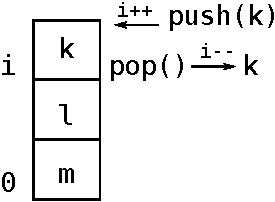
\includegraphics[scale=0.50]{fig/stack.pdf}
\end{center}
\end{wrapfigure}

\Question \label{ex:stack q2} Bonus. Write a \func{String} method which 
converts the stack to a string. This way you can print the stack using:
\lstinline{fmt.Printf("My stack %v\n", stack)}. This may aid in
debugging.
\end{Exercise}

\begin{Answer}

\Question 

\Question 

\end{Answer}


\begin{Exercise}[title={Var args},difficulty=5]
\label{ex:varargs}
\Question\label{ex:varargs q1}
Write a function that takes a variable numbers of \type{int}s and prints
each integer on a seperate line
\end{Exercise}

\draft{BETER}
\begin{Answer}
\Question
For this we need the \lstinline{...}-syntax so signal we have a
function that takes an arbitrary number of arguments.

\lstinputlisting[label=src:varargs,caption=A function with variable number of arguments]{ex-functions/src/var-arg.go}

\end{Answer}


\begin{Exercise}[title={斐波那契},difficulty=5]
\label{ex:fibonaci}
\Question\label{ex:fibonaci q1}
斐波那契数列以:$1, 1, 2, 3, 5, 8, 13, \ldots$ 开始。
或者用数学形式表达:$ x_1 = 1; x_2 = 1; x_n = x_{n-1} +
x_{n-2}\quad\forall n > 2 $。

编写一个函数,接受 \type{int} 值,并给出这个值得到的斐波那契数列。

\end{Exercise}

\begin{Answer}
\Question
下面的程序会计算出斐波那契数列。
\lstinputlisting[label=src:fib,caption=Fibonacci function in Go]{ex-functions/src/fib.go}

\showremarks
\end{Answer}


\begin{Exercise}[title={Map function},difficulty=4]
\label{ex:map function}
A \func{map()}-function is a function that takes
a function and a list. The function is applied to 
each member in the list and a new list containing
these calculated values is returned.
Thus: 
$$ map(f(), (a_1,a_2,\ldots,a_{n-1},a_n)) =  (f(a_1), f(a_2),\ldots,f(a_{n-1}), f(a_n)) $$
\Question \label{ex:map function q1} Write a simple
\func{map()}-function in Go. It is sufficient
for this function only to work for ints.
\Question \label{ex:map function q2} Expand your code to also work on a list of strings.

\end{Exercise}

\begin{Answer}

\Question 
\begin{lstlisting}[caption=A \func{Map} function]
func Map(f func(int) int, l []int) []int {
        j := make([]int, len(l))
        for k, v := range l {
                j[k] = f(v)
        }
        return j
}

func main() {
        m := []int{1, 3, 4}
        f := func(i int) int {
                return i * i
        }
        fmt.Printf("%v", (Map(f, m)))
}
\end{lstlisting}

\Question Answer to question but now with strings
\end{Answer}




\begin{Exercise}[title={Minimum and maximum},difficulty=0]
\label{ex:minmax}
\Question\label{ex:minmax q1} Write a function that finds the
maximum value in an \type{int} slice (\type{[]int}).

\Question\label{ex:minmax q2} Write a function that finds the
minimum value in an \type{int} slice (\type{[]int}).

\end{Exercise}

\begin{Answer}
\Question This function returns the largest int in the slice \var{l}:
\begin{lstlisting}
func max(l []int) (max int) {   |\longremark{We use a named return parameter;}|
        max = l[0]      
        for _, v := range l {   |\longremark{Loop over \var{l}. The index of the element is %
not important;}|
                if v > max {    |\longremark{If we find a new maximum, remember it;}|
                        max = v 
                }   
        }   
        return  |\longremark{A ``lone'' return, the current value of \var{max} is now returned.}|
}
\end{lstlisting}
\showremarks

\Question This function returns the smallest int in the slice \var{l}. It is almost identical to \func{max}:
\begin{lstlisting}
func min(l []int) (min int) {
        min = l[0]
        for _, v := range l { 
                if v < min {
                        min = v 
                }   
        }   
        return
}
\end{lstlisting}
The interested reader may combine \func{max} and \func{min} into one function with a selector
that lets you choose between the minimum or the maximum, or one that returns both values.
\end{Answer}


\begin{Exercise}[title={Bubble sort},difficulty=1]
\label{ex:bubble}
\Question\label{ex:bubble q1} Write a function that performs 
Bubble sort on slice of ints. From \cite{bubblesort}:
\begin{quote}
It works by repeatedly stepping through the list to be sorted, comparing each
pair of adjacent items and swapping them if they are in the wrong order. The
pass through the list is repeated until no swaps are needed, which indicates
that the list is sorted. The algorithm gets its name from the way smaller
elements ``bubble'' to the top of the list. 
\end{quote}

\cite{bubblesort} also gives an example in pseudo code:
\begin{lstlisting}[language=pascal]
procedure bubbleSort( A : list of sortable items )
  do
    swapped = false
    for each i in 1 to length(A) - 1 inclusive do:
      if A[i-1] > A[i] then
        swap( A[i-1], A[i] )
        swapped = true
      end if
    end for
  while swapped
end procedure
\end{lstlisting}
\end{Exercise}

\begin{Answer}
\Question 
The Bubble sort isn't terribly efficient, for $n$ elements it scales
$O(n^2)$. See QuickSort \cite{quicksort} for a better sorting algorithm.

But Bubble sort is easy to implement, the following is an example.
\lstinputlisting[caption=Bubble sort,linerange=4-19]{ex-functions/src/bubblesort.go}

Because a slice is a reference type the \func{bubblesort} function works and
does not need to return a sorted slice.
\end{Answer}


\begin{Exercise}[title={Functions that return functions},difficulty=1]
\label{ex:function}
\Question\label{ex:function q1} Write a function that returns a function
that performs a $+2$ on integers. Name the function \func{plusTwo}.
You should then be able do the following:
\begin{lstlisting}
p := plusTwo()
fmt.Printf("%v\n", p(2))
\end{lstlisting}
Which should print 4.
See section \titleref{sec:callbacks} on page \pageref{sec:callbacks} for information
about this topic.

\Question\label{ex:function q2} Generalize the function from \ref{ex:function q1},
and create a \func{plusX(x)} which returns a functions that add \var{x} to an
integer.
\end{Exercise}

\begin{Answer}
\Question
\begin{lstlisting}
func main() {
        p2 := plusTwo()
        fmt.Printf("%v\n",p2(2))
}

func plusTwo() func(int) int { |\longremark{Define a new function that returns a function. %
See how you you can just write down what you mean;}|
        return func(x int) int { return x + 2 } |\longremark{Function literals at work, %
we define the +2--function right there in the return statement.}|
}
\end{lstlisting}
\showremarks

\Question
Here we use a closure:
\begin{lstlisting}
func plusX(x int) func(int) int { |\longremark{Again define a function that returns %
a function;}|
        return func(y int) int { return x + y } |\longremark{Use the \emph{local} variable %
\var{x} in the function literal.}|
}
\end{lstlisting}
\showremarks
\end{Answer}


\cleardoublepage
\section{答案}
\shipoutAnswer
